The indicator layer will be responsible for the output of the system, where the indicator subsystem consists of an industrial light tower, which displays the status of the working cell.   

\subsection{Industrial Light Tower}
An industrial light tower system, typically used in a working cell or industrial setting, serves several essential responsibilities to ensure the efficient and safe operation of the workspace. The specific responsibilities of an industrial light tower system may vary depending on the application. For our system, it serves as an inference to the work environment as it indicates different modes with colored LEDs as get input from the controller and outputs as LEDs. 
\begin{figure}[h!]
	\centering
 	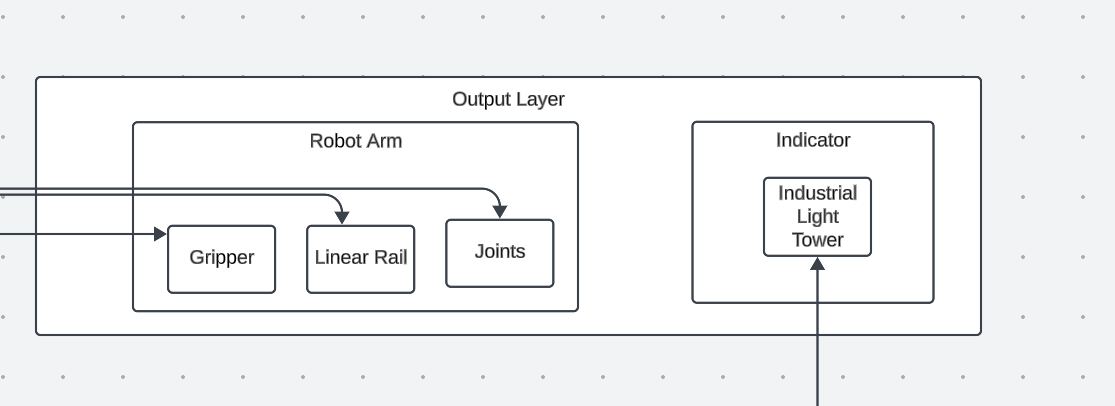
\includegraphics[width=0.60\textwidth]{images/indicator.png}
 \caption{Indicator subsystem description diagram}
\end{figure}

\subsubsection{Assumptions}
The "Indicator" subsystem assumes that it will receive status information from the Controller about the working status of the robot arm. It is assumed that this system will be a reliable communication source or interface to update the status of the working cell. 
\subsubsection{Responsibilities}
Signaling and Alerts: Industrial light tower systems often include signal lights or beacons. These lights can be used to convey information or alerts to workers or nearby personnel. Common signals include indicating when a machine is running, signaling the need for maintenance or repair, or warning of specific hazards or emergencies.

Status Indication: The light tower system can provide status indications for machines or equipment within the working cell. 

Safety: Ensuring the safety of workers is a primary responsibility. Light towers can be programmed to flash or change colors to draw attention to potential safety hazards, such as moving equipment or areas that require caution.

\subsubsection{Subsystem Interfaces}

\begin {table}[H]
\caption {Subsystem interfaces} 
\begin{center}
    \begin{tabular}{ | p{1cm} | p{6cm} | p{3cm} | p{3cm} |}
    \hline
    ID & Description & Inputs & Outputs \\ \hline
    \#01 & Stop operating & \pbox{3cm}{controller} & \pbox{3cm}{red led signal}  \\ \hline
    \#02 & Require caution & \pbox{3cm}{controller} & \pbox{3cm}{yellow led signal}  \\ \hline
    \#03 & Operating Mode & \pbox{3cm}{controller} & \pbox{3cm}{green led signal}  \\ \hline
    \end{tabular}
\end{center}
\end{table}

